\section{Architecture}
\label{sec:architecture}

In this section outlines the architecture of the Votes-System.
At first, we elaborate the design of its EJB-Module.
Following that, we briefly discuss the architecture of the War-Module.


\subsection{VotesEJB Architecture}
\label{subsec:votesejb-architector}
In order to maintain scalability, the business and persistence components of a JavaEE Web Application are packaged into EJB JAR Module.
Such modules can easily be cloned to handle more workload properly.
In general an EJB module consists of an domain model, an arbitrary amount of business and persistence classes and a facade, making the relevant components visible to the outside.

\subsubsection{The Votes Domain Model}
\label{subsubsec:the-votes-domain-model}
The Votes Domain Model specifies the structure and relations of its entities.
It is depicted in figure \ref{figure:ejb-model} and mostly matches the requirements defined in section §\ref{sec:requirements}.
However, we made some extensions:

\begin{figure}[h]
\centering
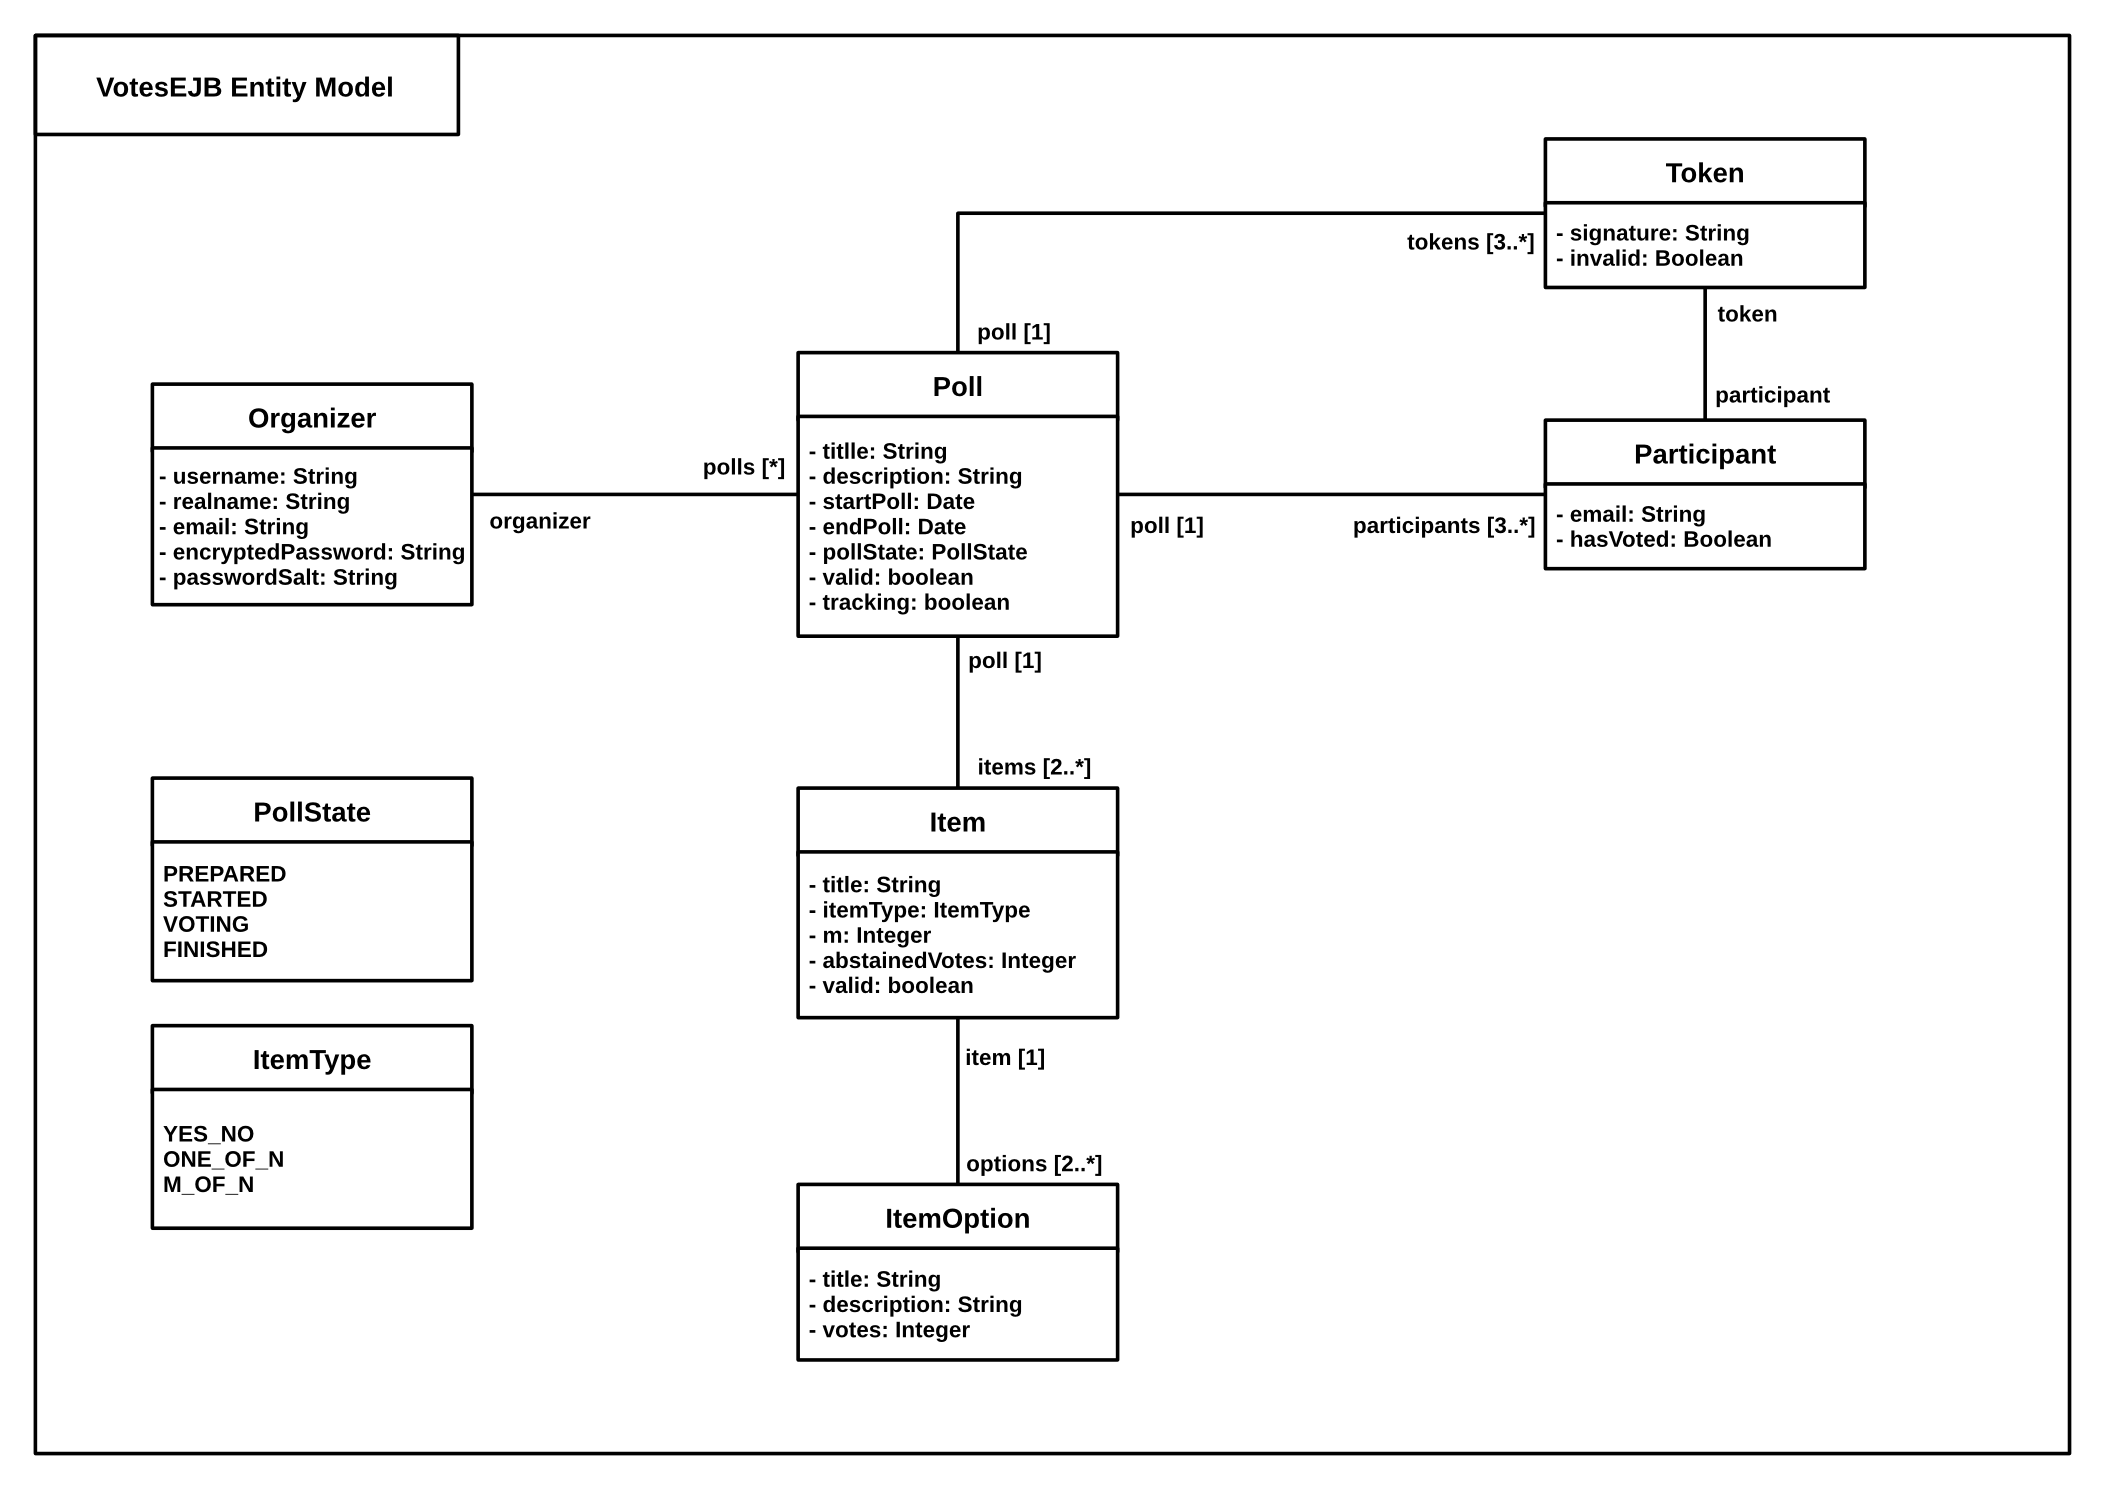
\includegraphics[width=0.7\textwidth]{png/ejb-model.png}
\caption{VotesEJB Entity Model}
\label{figure:ejb-model}
\end{figure}

\begin{itemize}

\item
Polls and Items have flag, which determines if they are valid.

\item
Items have a counter, which counts abstentions.

\item
ItemOptions have a counter, which counts the number of participants that have selected that said option.

\item
Tokens can be invalidated.

\item
Organizers also store a salt to strengthen password hashes.

\end{itemize}



\paragraph{Anonymity:}
The criterion of utmost importance for a voting system's quality is the degree of assured anonymity.
That means, at no point it must be possible to link a participant to his or hers voting decision.
Therefore certain restriction have been made:
\begin{itemize}

\item
Polls with less than three participants cannot be asserted anonymous, so poll has to have at leas three participants.

\item
Although the voting system records which participant has voted for administrative purposes, his or hers exact vote remains unknown to the data structure.
This is ensured by numeric option counters, which increase if a participant has selected an option.

\item
Token signatures act as ballots, which allow a participant to view polls and submit a vote. 
Such signatures must be hard to forge.
To assure this quality, signatures are type 4 UUIDs generated by \texttt{UUID.randomUUID()}\footnote{\url{http://docs.oracle.com/javase/7/docs/api/java/util/UUID.html}}.

\end{itemize}


\paragraph{Security:}
Another issue of importance is reflected by the domain model is the authentication of organizers.
To ensure that only the creators of polls can access their settings, organizer passwords cannot be stored in clear text.
In order to secure the database against attacks, we facilitate the comment technique of salted hashes to store passwords.
A password is stored as SHA-256 hash of its concatenation with a type 4 UUID salt.
The salt is stored alongside.


\subsubsection{Votes Entity Persistence}
\label{subsubsec:votes-entity-persistence}
The Java Persistence API (JPA) used by JavaEE Web Applications follow a persistence strategy, which maps entity classes to database tables.
That means for each entity in the domain model exists a corresponding table.
However, to ensure the uniqueness of row tuples, entities need to have an \texttt{id} property, which is missing in figure \ref{figure:ejb-model}.
Entities of the votes domain model inherit such a property from the class AbstractEntity, depicted in figure \ref{figure:ejb-abstract-entity}.

\begin{figure}[h]
\centering
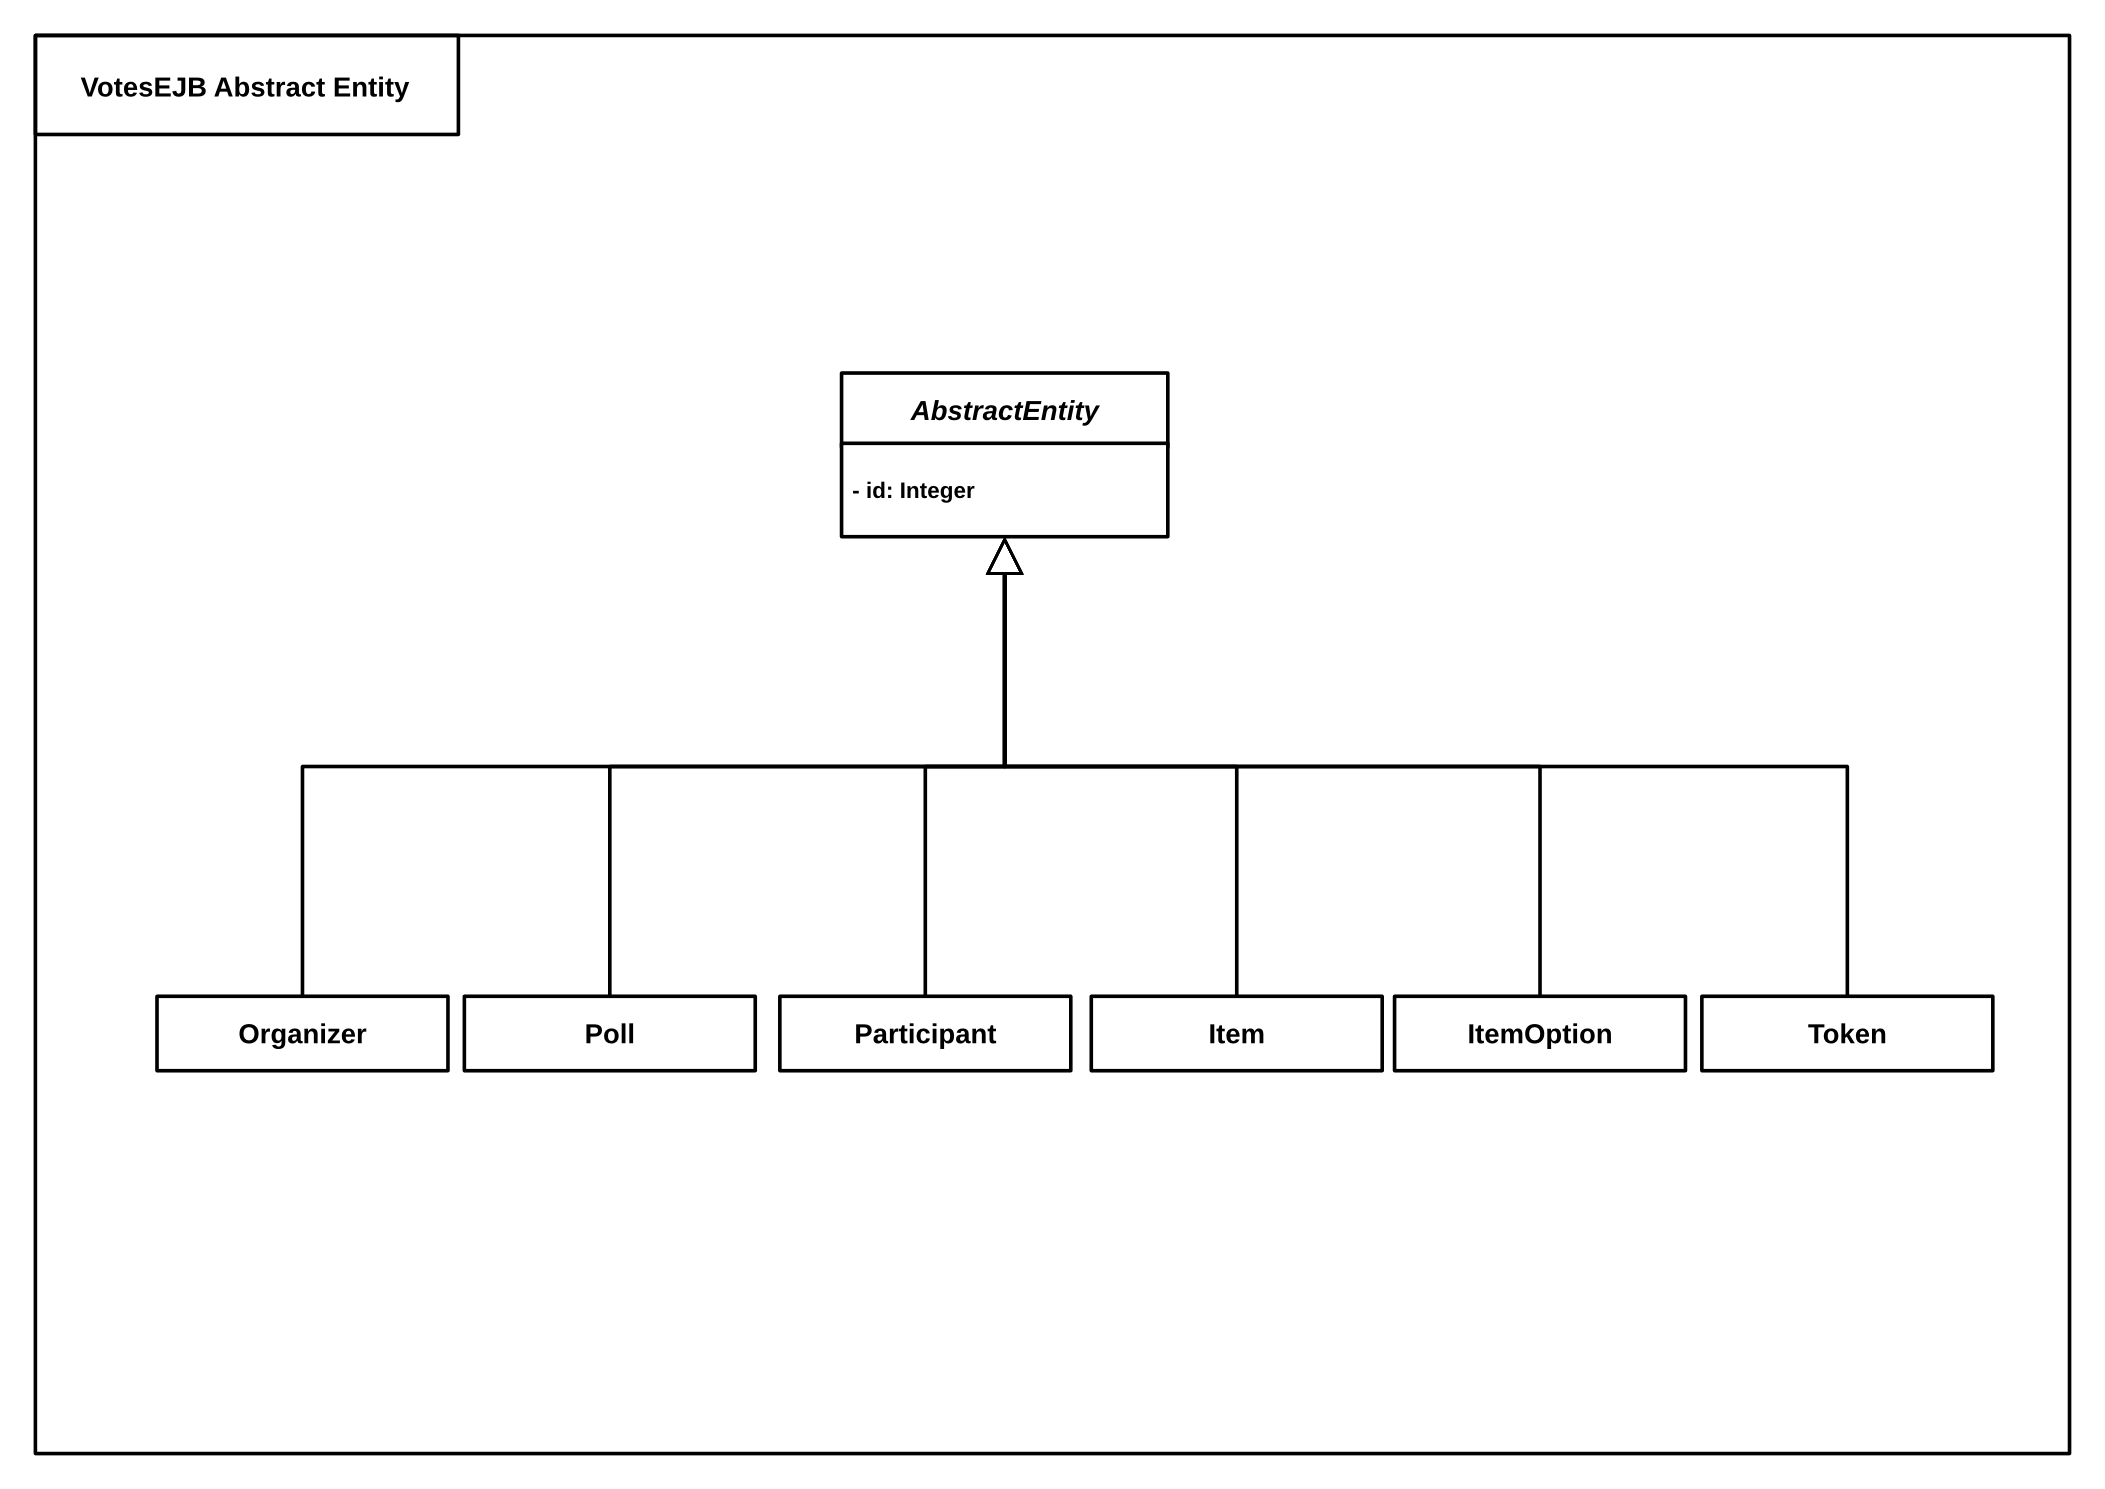
\includegraphics[width=0.7\textwidth]{png/ejb-abstract-entity.png}
\caption{VotesEJB Abstract Entity}
\label{figure:ejb-abstract-entity}
\end{figure}

Moreover, JPA encourages to use the \textit{Data Mapper}\footnote{\url{http://martinfowler.com/eaaCatalog/dataMapper.html}} pattern to handle persistence operations.
This pattern is exemplified in figure \ref{figure:ejb-data-mapper}, which shows the Poll entity class and its corresponding data mapper PollAccess.

\begin{figure}[h]
\centering
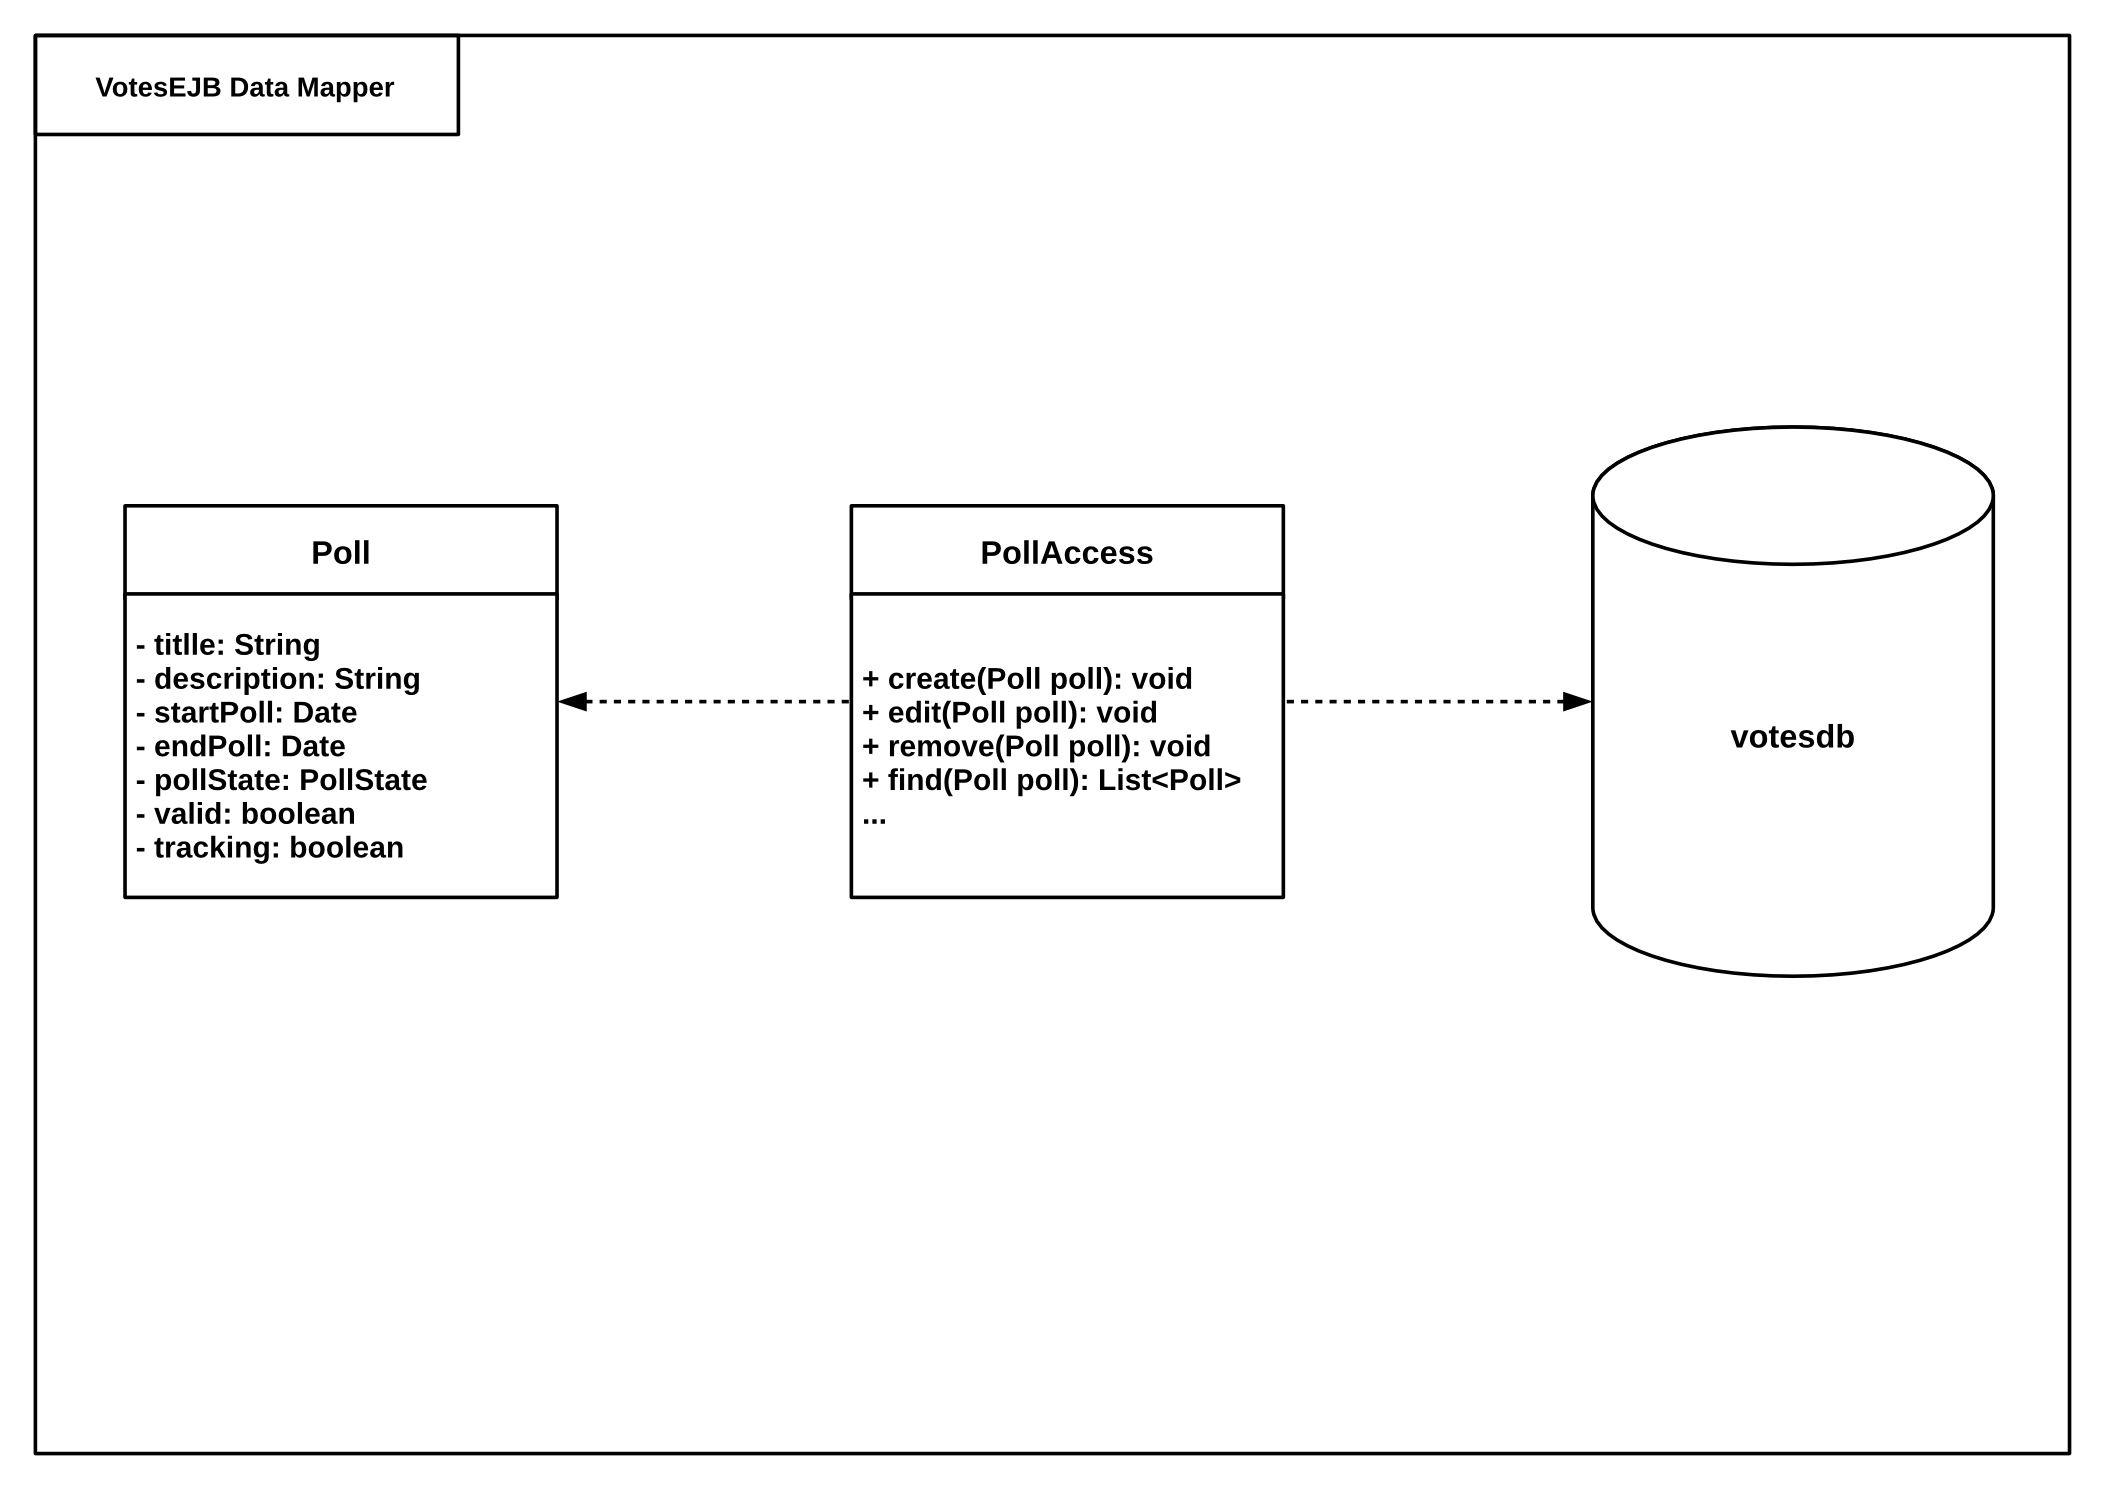
\includegraphics[width=0.7\textwidth]{png/ejb-data-mapper.png}
\caption{VotesEJB Data Mapper}
\label{figure:ejb-data-mapper}
\end{figure}

Each entity of the votes domain model has its own data mapper handling creation, reading, update and deletion of instances in the database.
Thus, this pattern decouples persistence structure from persistence behaviour. 
Mappers or Data Access Objects are also enhanced to do more complex database operations.

\subsubsection{The Votes Business Model}
\label{subsubsec:the-votes-business-model}
Besides the CRUD operations of the persistence layer, the Votes-System has scarcely any business logic.
One notable exception is the transition of poll states depicted in figure \ref{figure:poll-states}.

\begin{figure}[h]
\centering
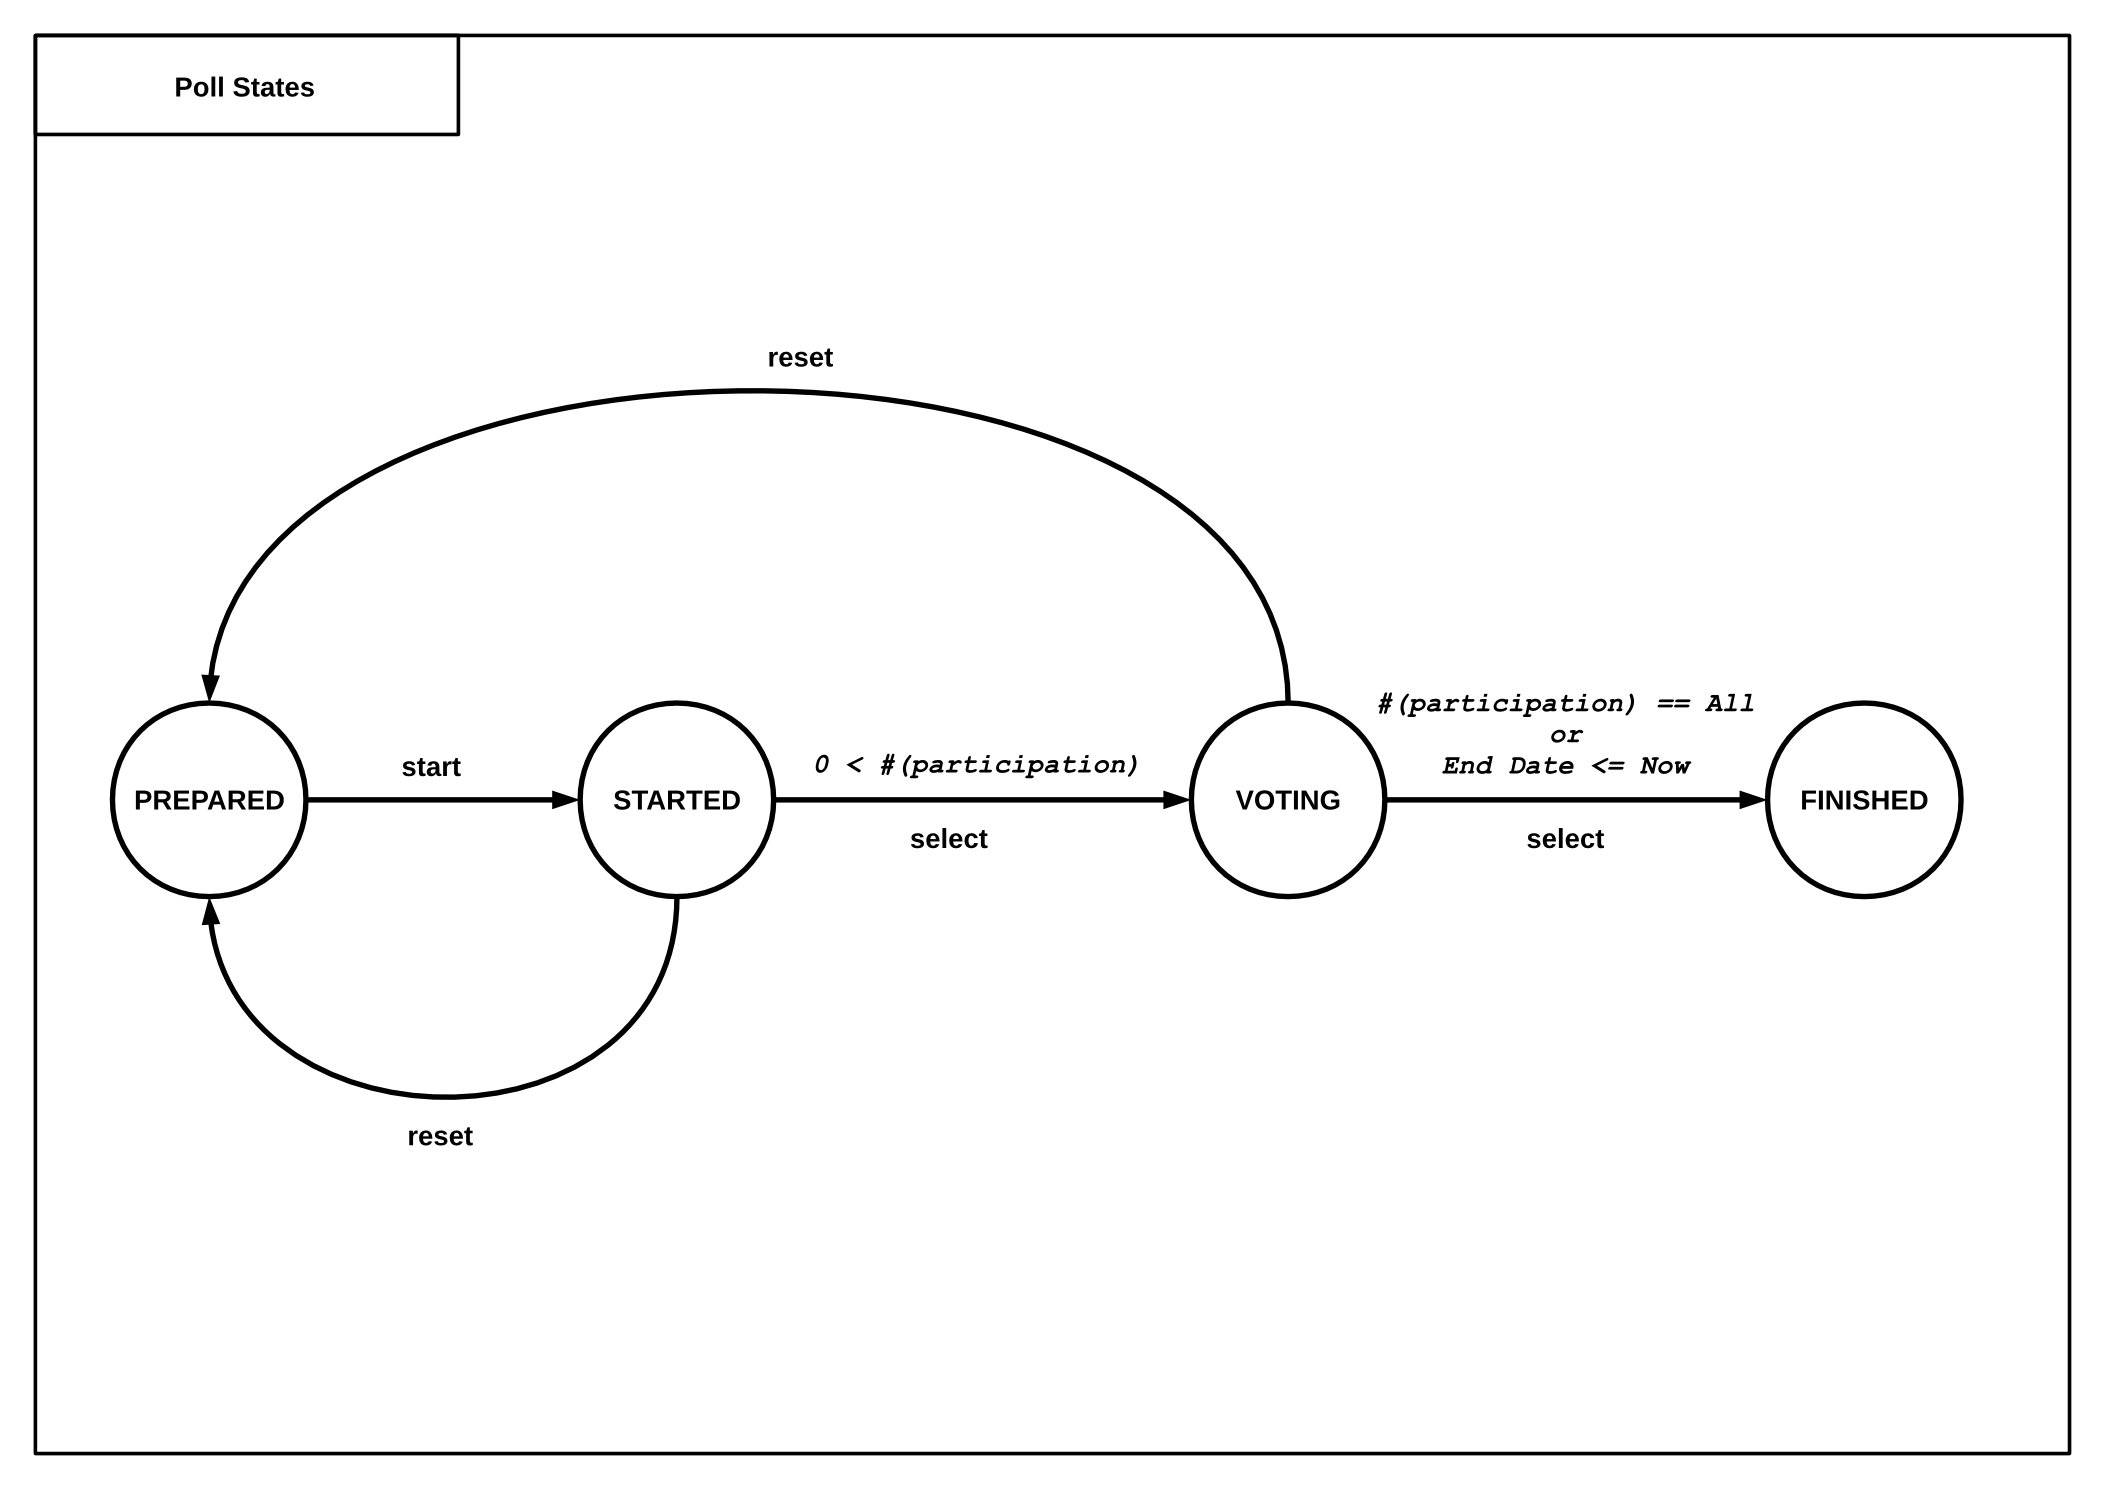
\includegraphics[width=0.7\textwidth]{png/poll-states.png}
\caption{Poll States}
\label{figure:poll-states}
\end{figure}

Poll states are frequently updated when either an organizer or participant access a certain poll.
Per default, a poll is created in state \texttt{PREPARED}.
If its organizer actively starts the poll, the state changes to \texttt{STARTED}.
This will trigger the sending of notification mails to all participants.
As soon as the first participant has submitted his or her vote the poll state changes to \texttt{VOTING}.
In either poll state \texttt{STARTED} or \texttt{VOTING} the organizer can reset the poll.
However, this will result in the deletion of all submitted votes so far.
When all participants have submitted their votes or the poll period is expired, the poll state changes to \texttt{FINISHED}.
This is the final state of poll.
If this state is reached, no further modification is possible.

\begin{figure}[h]
\centering
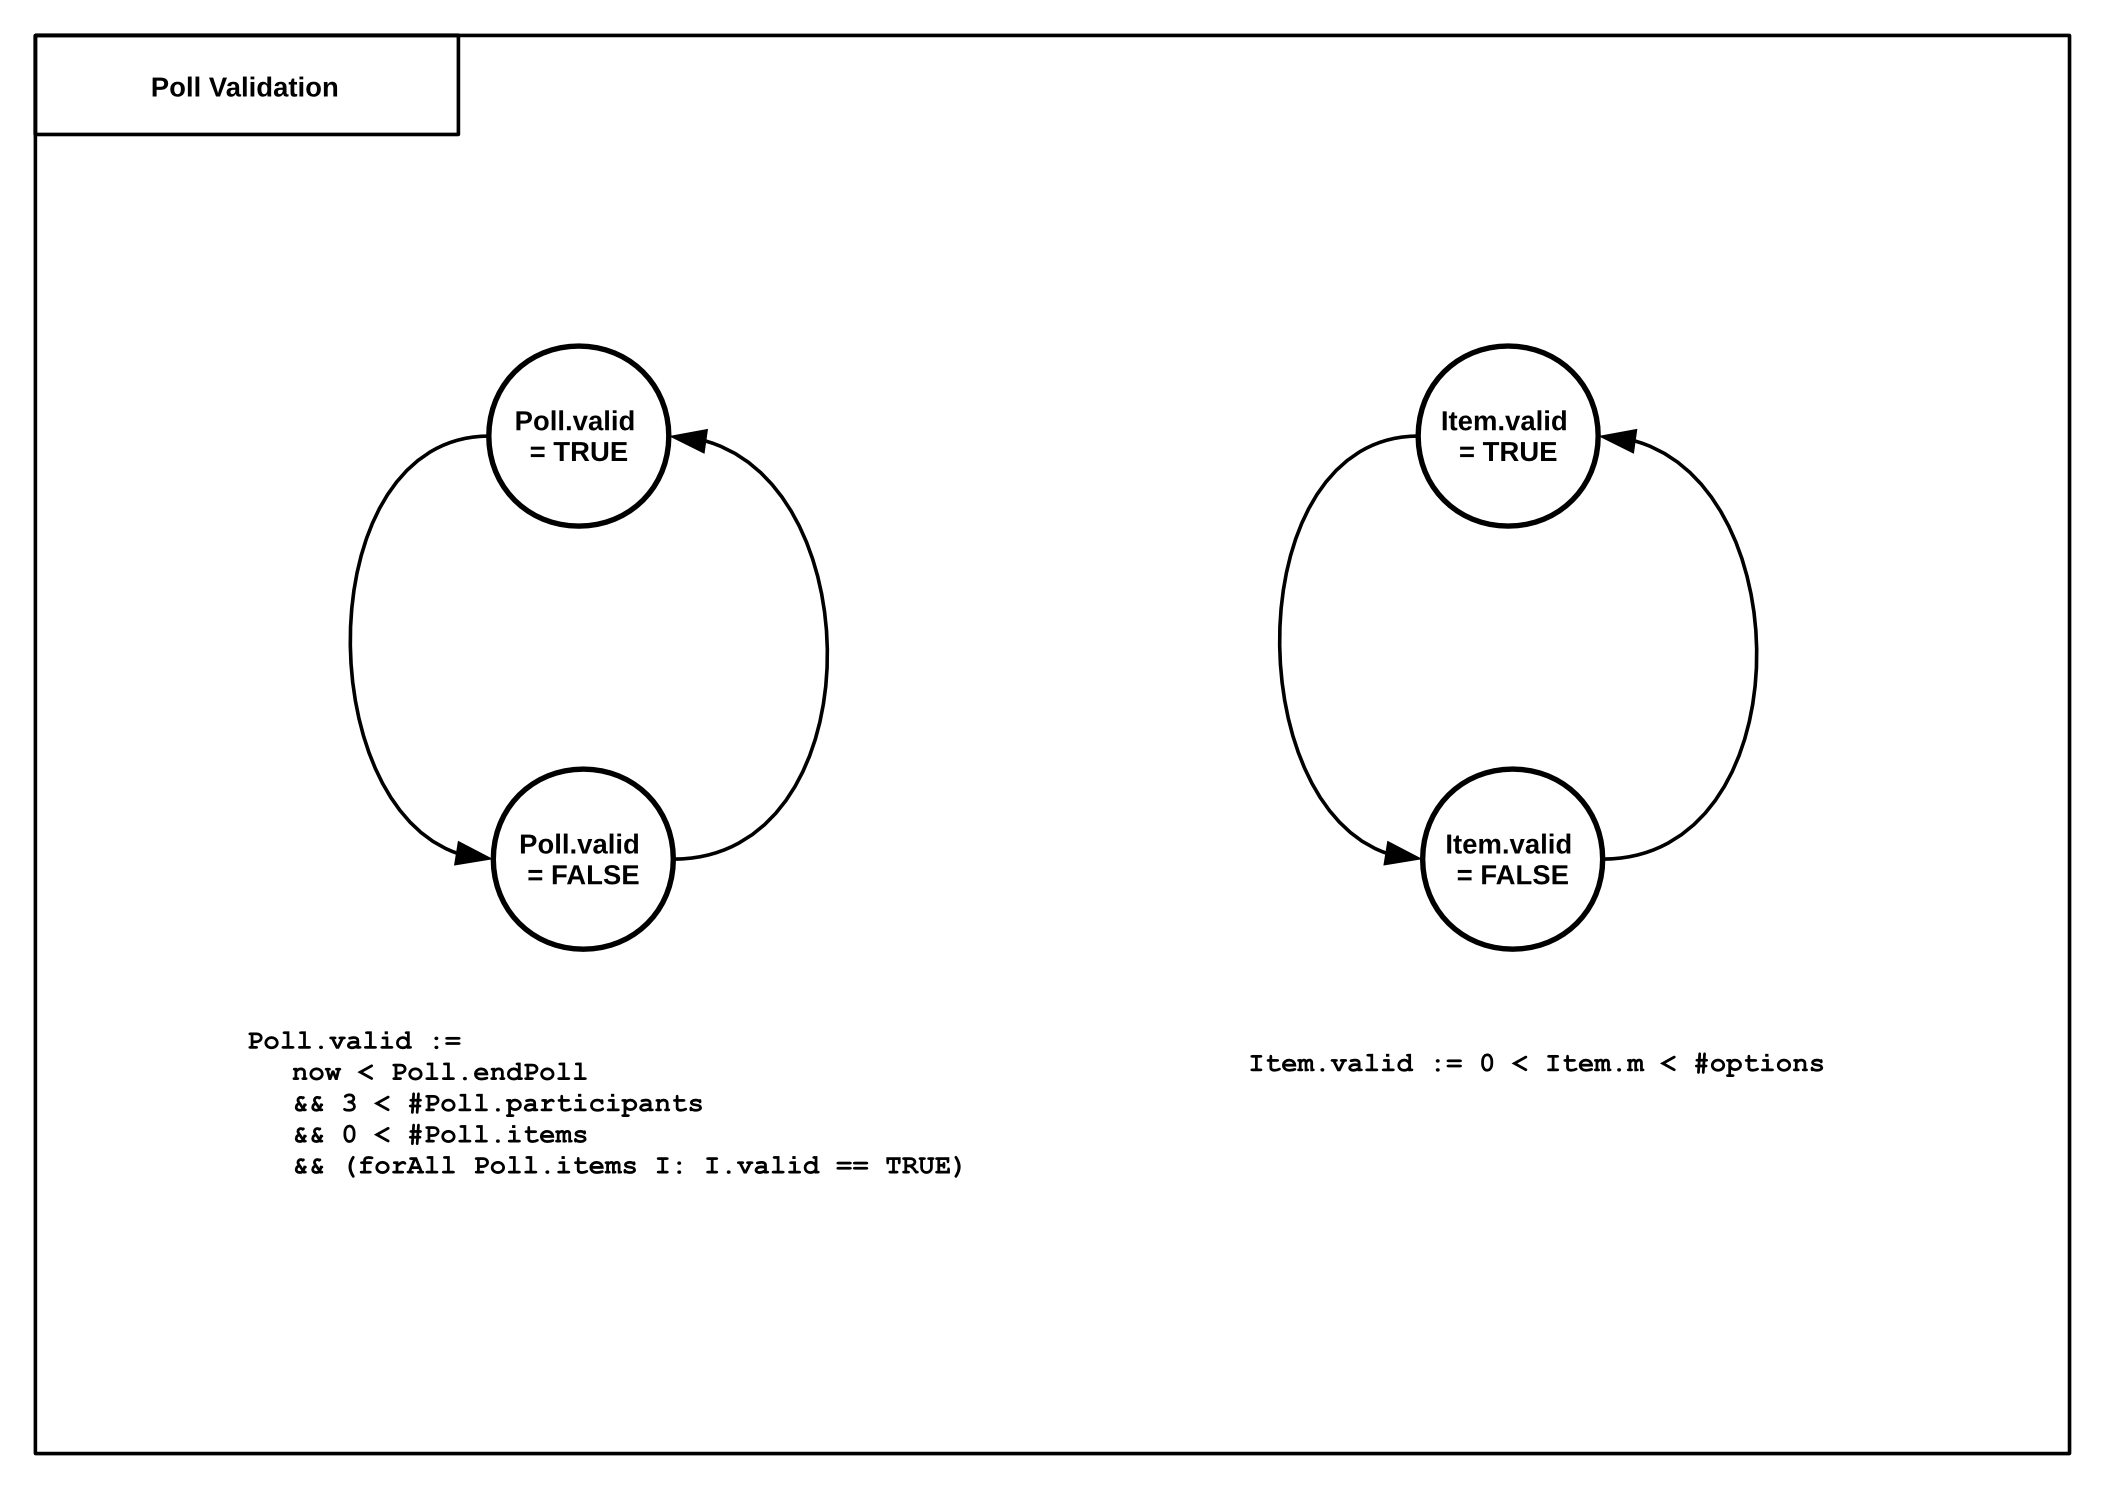
\includegraphics[width=0.7\textwidth]{png/poll-validation.png}
\caption{Poll Validation}
\label{figure:poll-validation}
\end{figure}

Another notable exception is the validation of polls, depicted in figure \ref{figure:poll-validation}.
Poll validation is one mean to ensure anonymity as only valid polls can be started.
Like the poll state, the poll valid flag is frequently updated when a poll is accessed.

However, such business operations are still closely related to CRUD.
So they are no additional business classes or packages besides the EJB facade, which is described in the following section.

\subsubsection{The VotesEJB Facade}
\label{subsubsec:the-votesejb-facade}
Additionally to the data mapper pattern, JPA also makes use of the \textit{Facade}\footnote{\url{http://en.wikipedia.org/wiki/Facade_pattern}} pattern.

\begin{figure}[h]
\centering
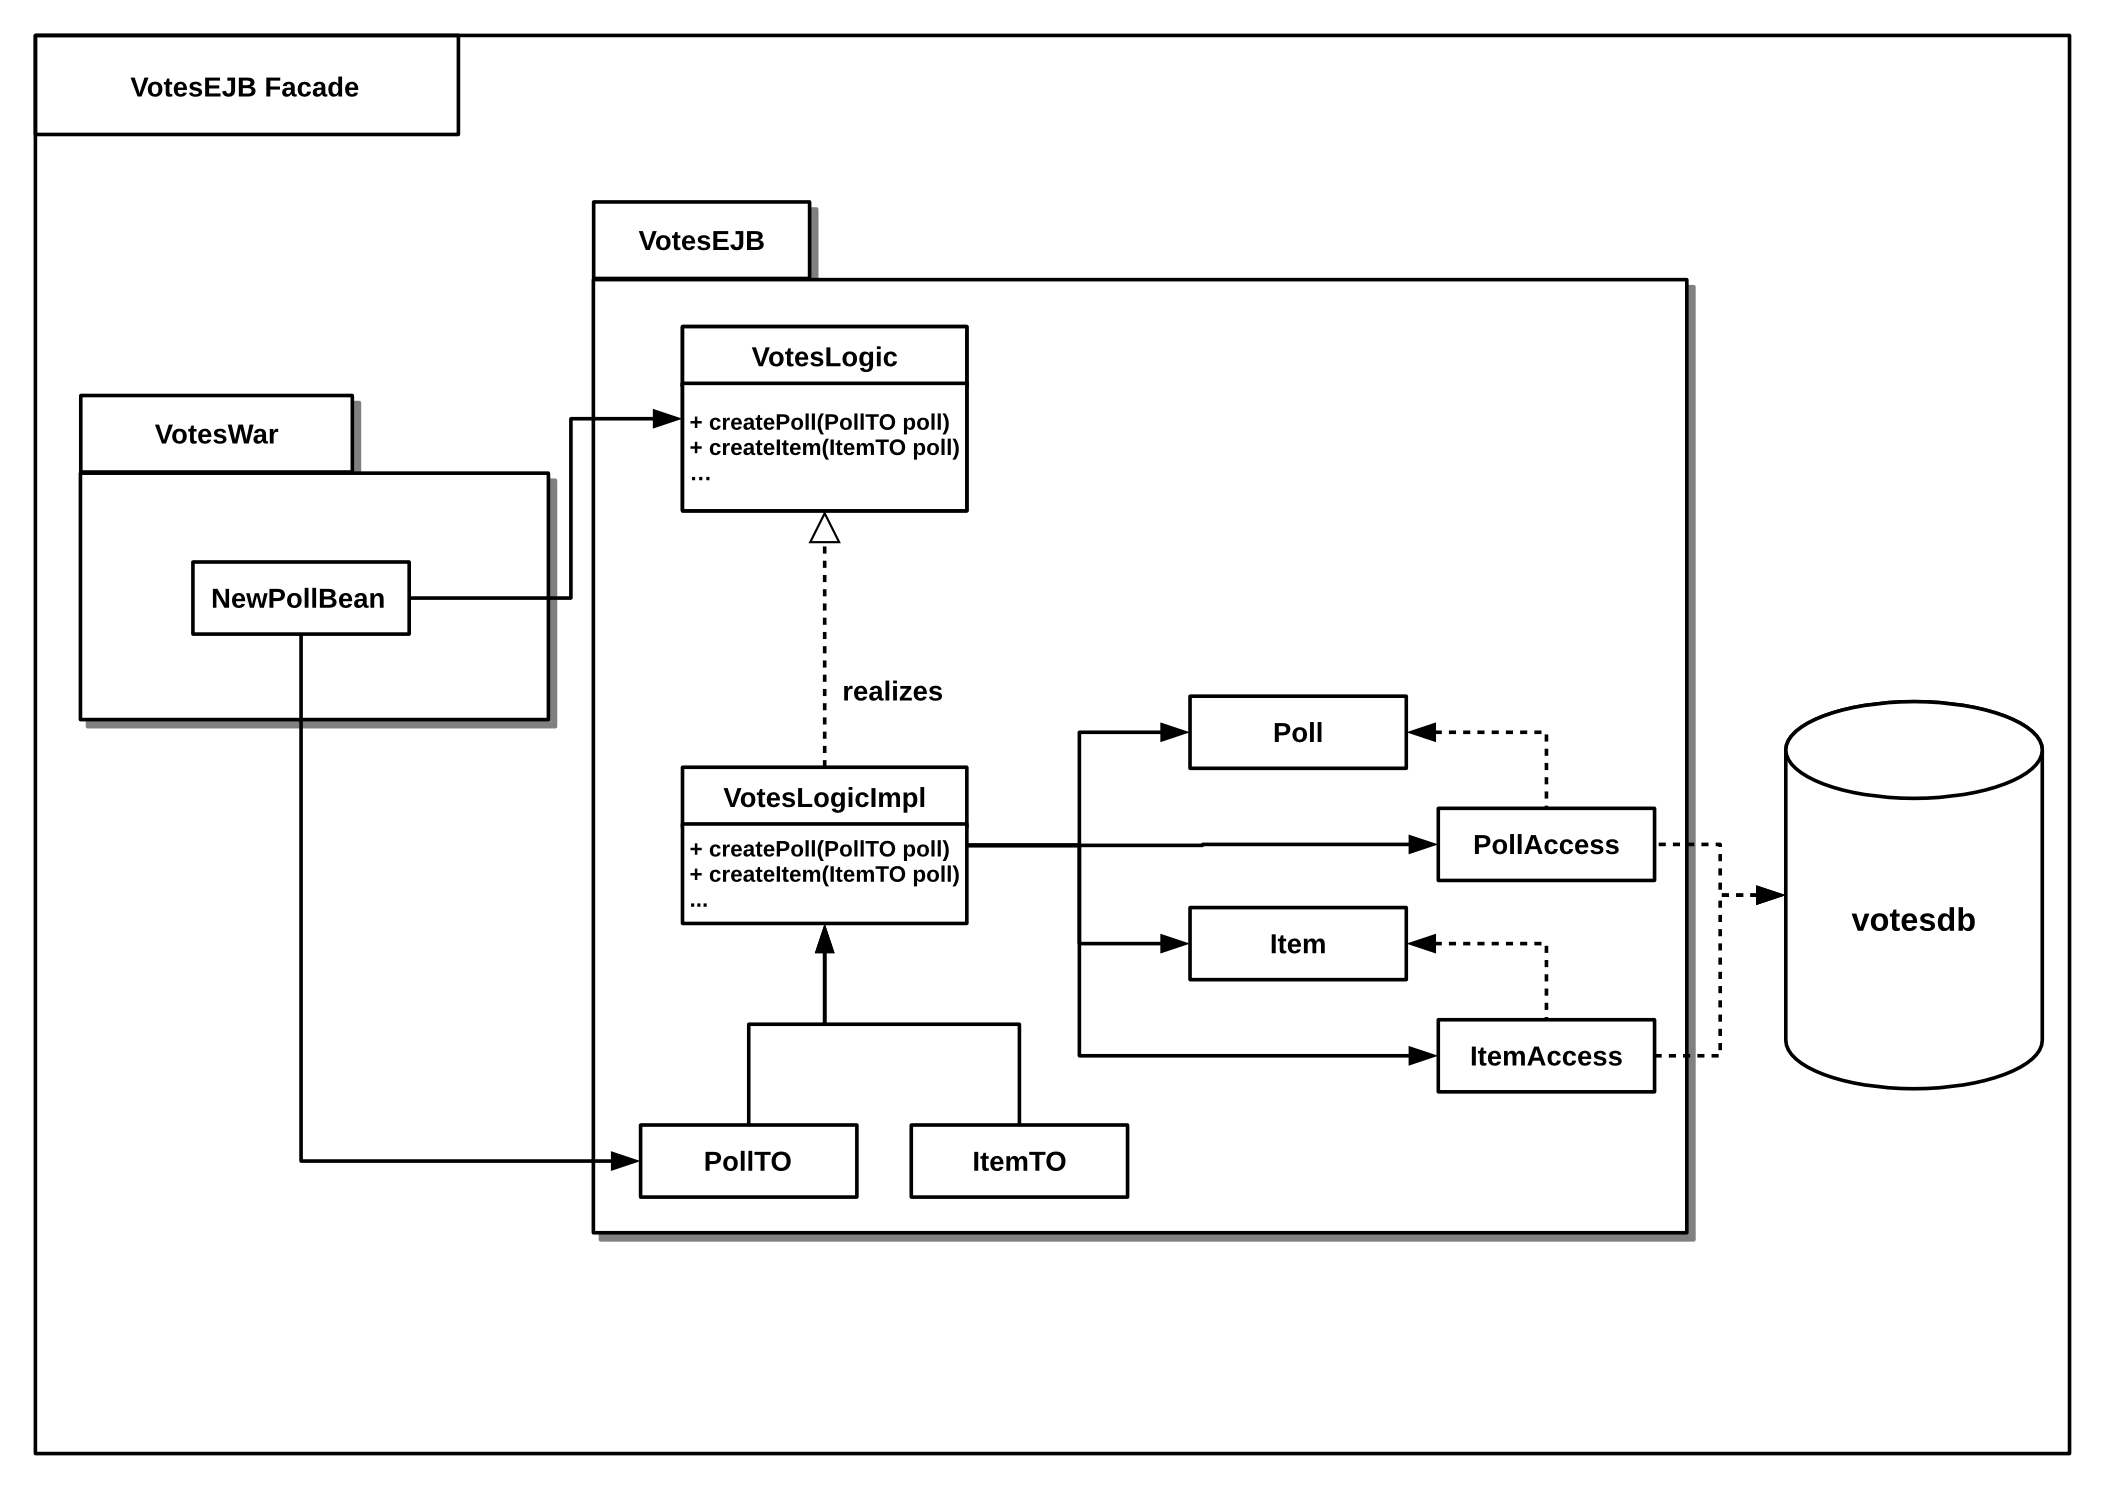
\includegraphics[width=0.7\textwidth]{png/ejb-facade.png}
\caption{VotesEJB Facade}
\label{figure:ejb-facade}
\end{figure}


%\subsection{Content Model}
%The following perspective describes the systems content model derived from requirement analysis model. The viewpoint is defined in \cite{Uwe08,uweref}, disregarding of the definition, the view is conform to a regular class diagram and does not use any stereotypes. Model elements for behaviour (like Operations) are not contained in this perspective.
%
%The votes content model can be seen in figure \ref{content_model}. The corresponding implementation serves as backbone of the running application in form of keeping the data and persisting it on a database. Later this is realises by JPA. Importance comes to the fact that no presentation details are included in the model, only the domain knowledge is included. The six classes represent all essential entity types that are involved in the requirements and their corresponding properties. Two enumeration types serve as additional datatypes. 
%
%High value comes to this view due to the fact that it can be directly mapped on the JPA and the transfer object classes that are part of the systems implementation. Apart from the fixed nature of the content model, described in the current requirements, a derivation process defining the Java classes can be of high good for further evolution and maintenance providing constructive quality assurance.
%
%
%
%\begin{figure}
%\centering
%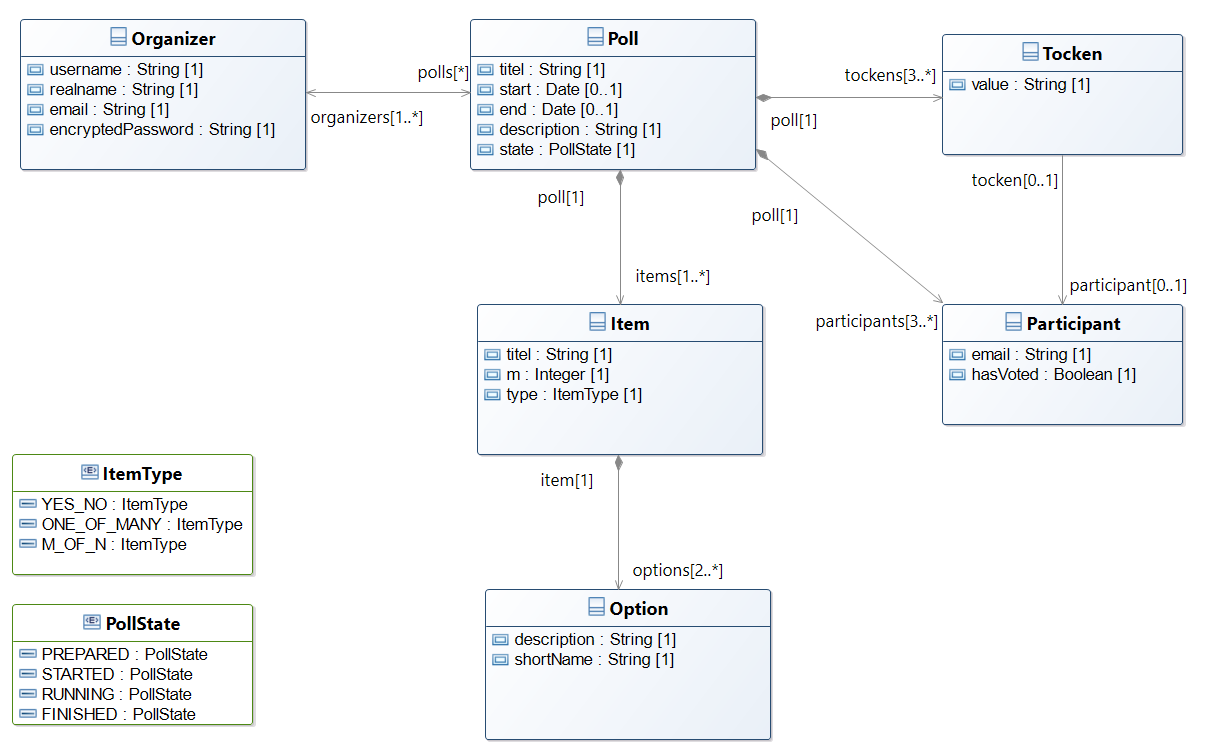
\includegraphics[width=1.0\textwidth]{png/domain_model.png}
%\caption{Votes content model}
%\label{F:content_model}
%\end{figure}
%
%
%\subsection{Navigation model}
%% Max has to check the models that.
%The navigation through the system and the interaction between user and content model is realised in html. The following model presented in figure \ref{F:navigation_model} focuses on the possible navigation paths. To define this on an abstract level we will coarsely stick to navigation model viewpoint defined by the UWE approve \cite{Uwe08,uweref}. It defines possible ways through the system by specifying different node types and one navigation links on the basis of UML stereotypes. A node is the smallest unit where any user can navigate to but more than one node can be presented on a single web page. Links are used to connect nodes and enable transitions, containment relations points out the structural containedness of one node in another.
%
%\begin{figure}
%\centering
%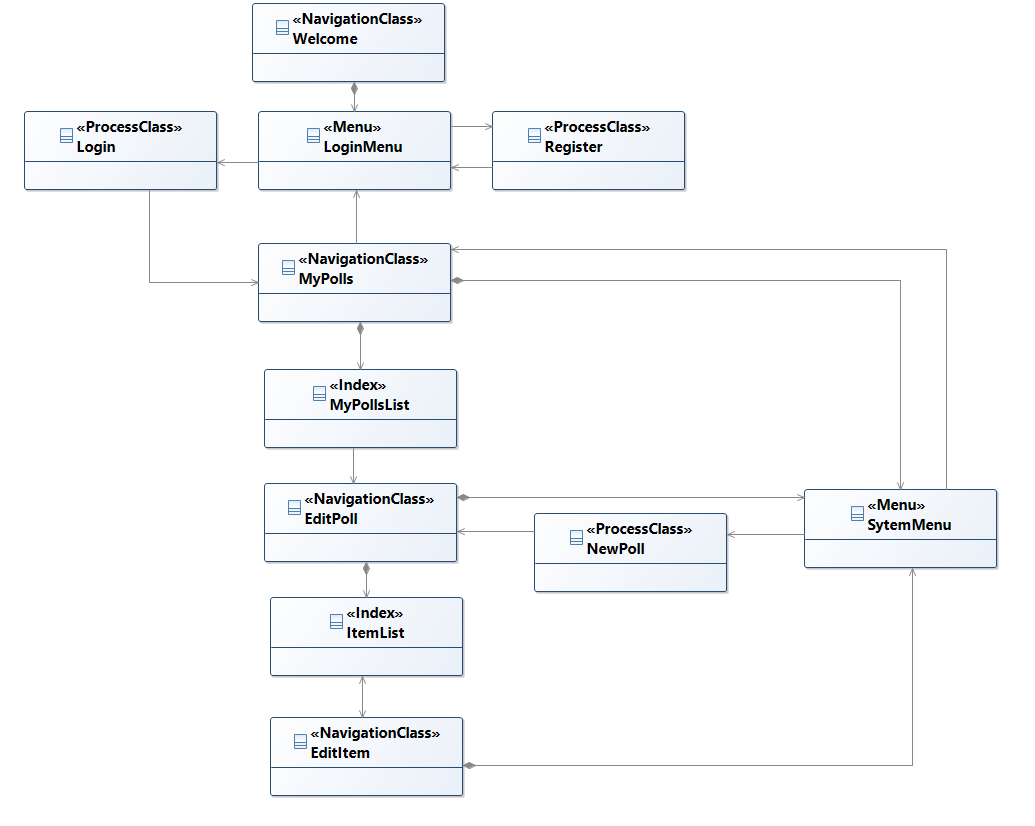
\includegraphics[width=1.0\textwidth]{png/navigation_model.png}
%\caption{Votes navigation model}
%\label{F:navigation_model}
%\end{figure}
%
%\subsection{Presentation model}
%% If we insert the UWE Presentation model, i need help of max because i can not undesand html jsf.
%
%The presentation model describes the components involved in the user interface and their relations. In the following model, displayed in figure \ref{F:presentation_model}, and its realisations web page, plotted in \ref{F:presentation_model_realisation}, the underlying structure is pointed out by using the example of the 'My Polls' page. The page consists of two parts and is defined by the component type MyPolls. The lower region holds one list displaying polls, the upper side displays the menu that allows the user to go back to the 'My Polls' page or to create a new Poll. In the case of the 'My Polls' type the left button of the SystemMenu part links back to the page itself. This is necessary because the SystemMenu type is also used in other context where it is needed to have a link back to the 'My Polls' page. Other pages of the votes system can be defined in similar fashion. The visual UWE stereotypes are missing in this model because of technical reasons.
%
% 
%\begin{figure}
%\centering
%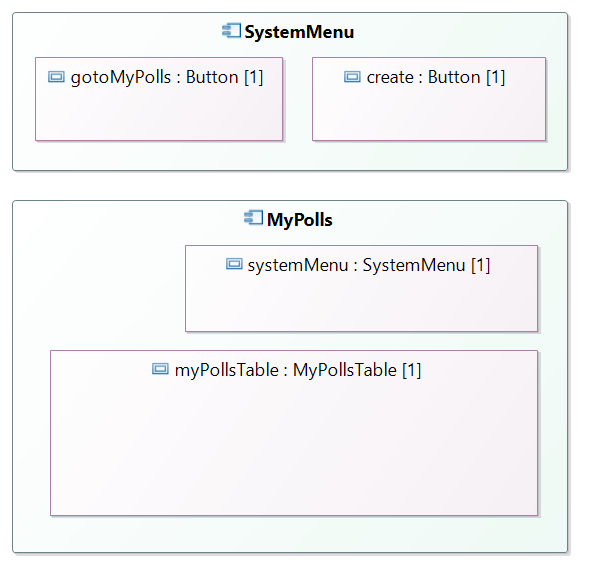
\includegraphics[width=0.4\textwidth]{png/presentation_model.png}
%\caption{Votes presentation model of 'My Polls' page}
%\label{F:presentation_model}
%\end{figure}
%
%\begin{figure}
%\centering
%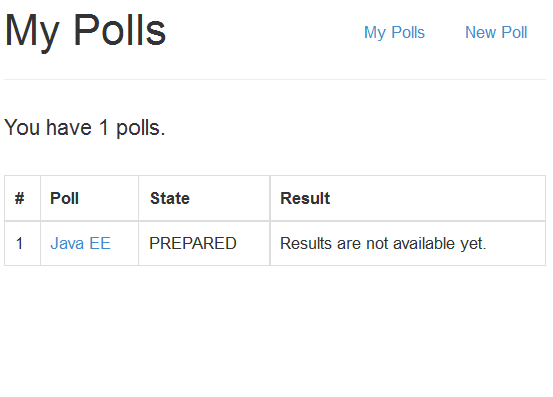
\includegraphics[width=0.4\textwidth]{png/presentation_model_realisation.png}
%\caption{Votes realisation of 'My Polls' page}
%\label{F:presentation_model_realisation}
%\end{figure}

\subsection{VotesWar Architecture}
% Do you mean packaging?